\documentclass[
 aip,
 jmp,
 amsmath,amssymb,
 reprint,
]{revtex4-1}
\usepackage{graphicx}
\usepackage{grffile}
\usepackage{dcolumn}
\usepackage{bm}
\usepackage{multirow}
\usepackage{color}

\newcommand{\massa}{{\large \textsc{massa}}}
\newcommand{\mass}{{\large \textsc{mass}}}
\newcommand{\figgus}{{\large \textsc{figgus}}}


\begin{document}
\preprint{AIP/123-QED} 

\title{Psychophysics of musical elements in discrete-time representation of sound}

\author{Renato Fabbri}
 \homepage{http://www.estudiolivre.org/el-user.php?view\_user=gk}
 \email{renato.fabbri@gmail.com}
  \affiliation{ 
Instituto de F\'isica de S\~ao Carlos, Universidade de S\~ao Paulo (IFSC/USP)
}

\author{Luciano da Fontoura Costa}
  \homepage{http://cyvision.ifsc.usp.br/~luciano/}
  \email{ldfcosta@gmail.com}
 \altaffiliation[Also at ]{IFSC-USP}

 \author{Osvaldo N. Oliveira Jr.}
  \homepage{www.polimeros.ifsc.usp.br/professors/professor.php?id=4}
  \email{chu@ifsc.usp.br}
 \altaffiliation[Also at ]{IFSC-USP}

\date{\today}
\begin{abstract}

    The representation of the basic elements of music - such as notes, ornaments and intervalar structures - in terms of discrete audio signal is often used in software for music creation and design. Nevertheless, there is no unified approach that relates these elements to the sound discrete samples. In this article, each musical element is described by equations in sonic time samples, which are all implemented in scripts within an open source software toolbox, referred to as \massa\ (Music and Audio in Sequences and Samples). The fundamental element, the musical note with duration, volume, pitch and timbre, is related quantitatively to the characteristics of the discrete-time signal. Internal variations, such as tremolos, vibratos and spectral fluctuations, are also considered, which enables the synthesis of notes inspired by real instruments and new sonorities. With this representation of notes, resources are provided for the generation of musical structures, such as rhythmic meter, pitch intervals and cycles. The efficacy of these physical descriptions of basic musical elements was confirmed by the synthesis of small musical pieces within each frame: basic notes, incremented notes and notes in music. It is possible to synthesize whole albums through collage of the scripts and parameterization. 
    The sample-based analitical description, and the paradigm of open source implementation, enables cientific experiments in precise and trustful ways. In fact, \massa\ has already been employed by external users for diverse purposes. Among these, it is mentioned an acoustic effect recognized by diverse individuals in mailing lists but not found in literature, and uses related to art and education.

\end{abstract}
\pacs{*43.66.-x,43.66.+y,05.10.-a} % PACS, the Physics and Astronomy
\keywords{psychophysics, acoustics, statistics, signal processing, digital audio, music}
\maketitle

\section{\label{sec:level1}Introduction}

Representing musical structures and artifices by it's discrete sound characteristics is the purpuse of this work. The results include mathematical relations and it's computer program implementations. Next section exposes the theoretical description, which is implemented as scripts in a one-to-one relation to the equations.

\subsection{Sound and digital audio}

Sound is a longitudinal wave of mechanical pressure. The frequency bandwidth between $20Hz$ and $20kHz$ is appreciated by human hearing system with boudaries dependent on the person, climate conditions and sonic charachteristics itself~\cite{Roederer}. If considereded the speed of sound of $\approx 343.2 m/s$, this limits corresponds to $\frac{343.2}{20} = 17.16\,m$ and $\frac{343.2}{20000}=17.16\,mm$.

Human perception of sound envolves captivation by bones, stomach, ears, tranfer functions of head and processing dorso and nervous system. Besides that, the ear is a dedicated organ to the capture of this waves. Its mechanism decomposes sound into its sinusoidal spectrum and delivers them to the nervous system. This sinusoidal components are crucial to musical fenomena, as one can observe in the composition of sounds with musical interest and in tunnings and scales. Subsection~\ref{subsec:dicNote} exposes the presence of sinusoids in discrete-time audio and charachterizes a basic musical note.

The representation of sound is called audio (although these terms are often used without distinction), and this can be provenient from caption by microphones or from sythesis. Often enough, digital audio is specified by protocols that eases file storage and transfering, in cost of a direct representation or even some loss in quality. Standard representation of digital audio, on the other hand, consists of samples equally spaced by $\lambda_s$ durations in time, with each sample spacified by a sample number of bits. This is called the Pulse Code Modulation representation of sound (PCM). A PCM digital sound is charachterized by it's sampling frequency $f_s=\frac{1}{\lambda_s}$, also called sampling rate, and bit depth, which is the number of bits used of representing the amplitude of each sample. Figure~\ref{fig:PCM} shows $25$ samples of a PCM áudio with $4$ bits each. The $2^4=16$ steps for each sample, together with the regular spacing $\lambda_s$ between them, introduces a quantization error. This noise, caused by this errors, diminishes as these spacing diminishes.


\begin{figure*}
    \centering
        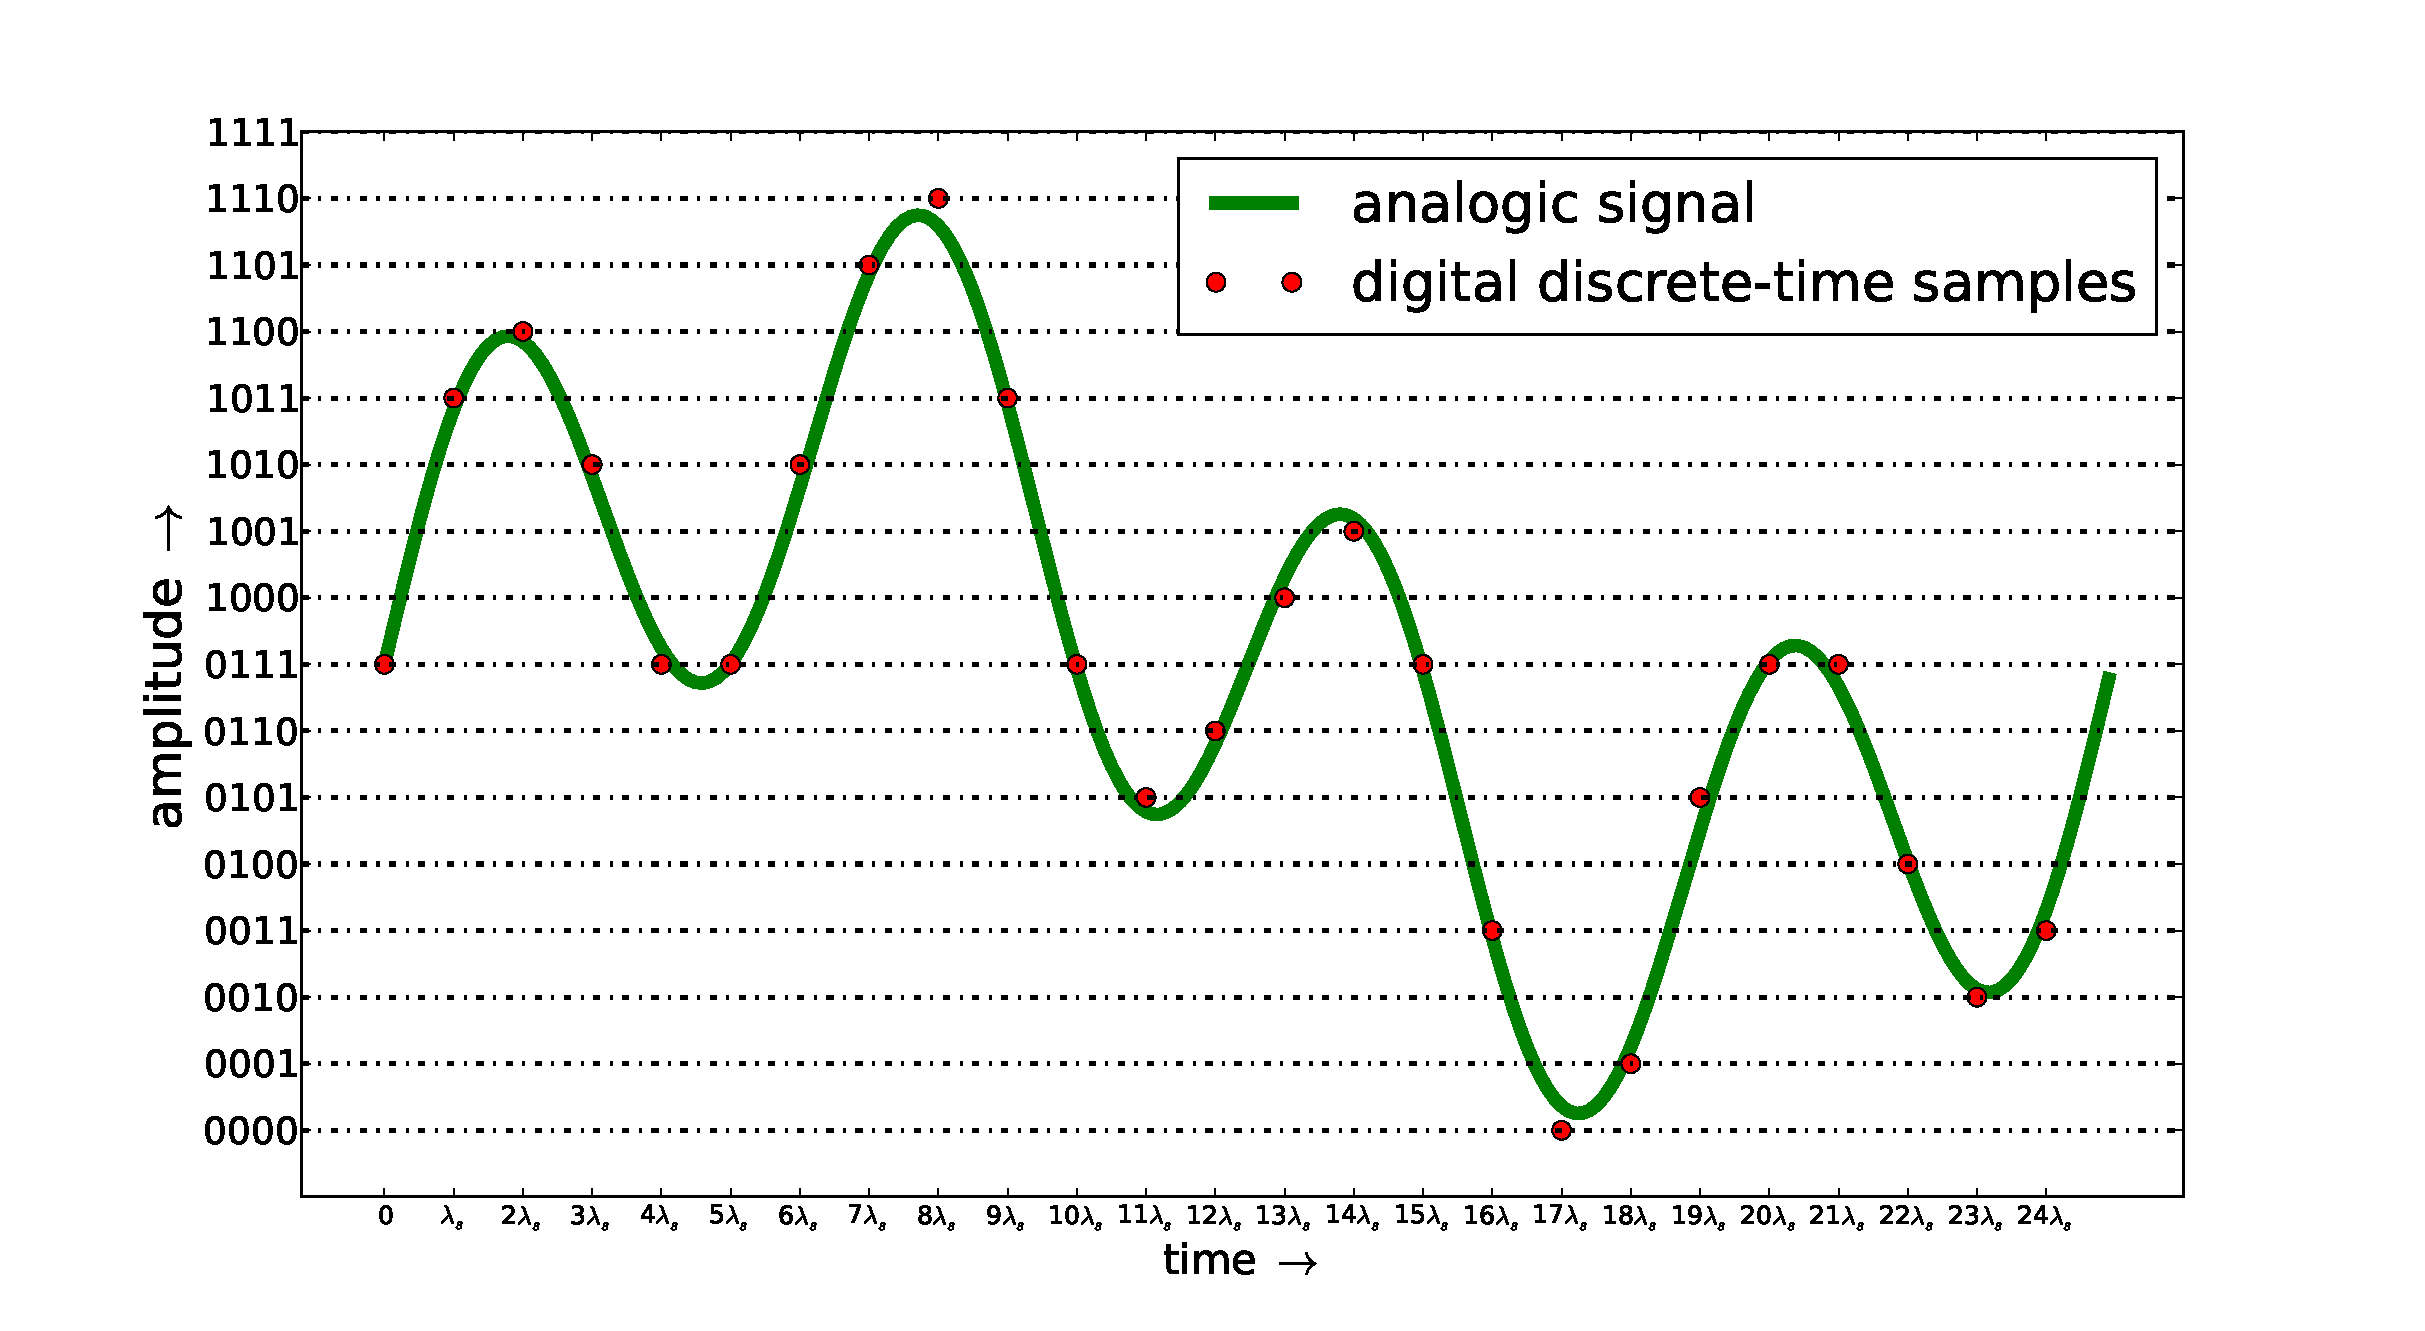
\includegraphics[width=\textwidth]{figures/pcm}
        \caption{Pulse Code Modulation (PCM) audio: an analogic signal is represented by 25 samples with 4 bits each.}
        \label{fig:PCM}
\end{figure*}




By the Nyquist theorem, it is known that half the sampling frequency is the maximum frequency of the signal. Thus, it is necessary to have a sampling frequency at least twice the highest frequency heard by humans $f_s \geq 2\times 20kHz = 40kHz$. This is the basis for the use of the sampling frequencies $44.1kHz$ and $48kHz$, standards in Compact Disks (CD) and Broadcast systems (Radio and TV), respectively.

\subsection{Sonic art and musical theory}

A common definition for music is art in sound and silence. For the average listener - and a reasonable part of specialists -the notion of music presupposes rythmic and pitch organization such as explained in subsection~\ref{subsec:notesMusic}. Music from the twentieth century enlarged this traditional comprehension of music. This occured in concert music, specially in the concrete, electronic and electroacoustic styles. On the last decade of the century, it was evident that popular music has also incorporated sounds without defined pitch and temporal organization out of simple metrics. Even though, the note stands paradigmatic as a 'fundamental unit' of musical structures and, in practice, it can unfold in sounds that observe this recent developments. The definition and expansion of the musical note as the fundamental unit of music is approached in subsections~\ref{subsec:discNote} and~\ref{subsec:internalVar}, respectively. Subsection~\ref{subsec:notesMusic} tackles the organization of musical notes in a higher level~\cite{Wisnick,Webern,Lerdhal,Cook,Lacerda}.

Musical theory embody topics as diverse as psicho-acoustics, cultural manifestations and formalisms. The section~\ref{sec:results} point this topics as needed and designate external complements~\cite{Zamacois,Schoenberg,microsound}.

\subsection{Computational implementation}
The results presented in this article are implemented inf the form of scripts, i.e. small programs for better availability and validation of the models as acessible techology.  This constitute the \massa\ toolbox, available in public domain in an open Git repository~\cite{gitBook}. This scripts are written in Python and make use of external libraries Numpy and Scikits/Audiolab that performs calls to Fortran routines for better computational efficiency. Part of this code has been trascribed to JavaScript and native Python with readiness, what points to uses of this contribution in web browsers such as Firefox and Chromium~\cite{numpy, audiolab, tutpython, python}.

This are all open technologies, that is, published in licenses that allows copy, distribution and use of any part for research and derivatives. This way, the work here presented is available and eases co-authorship processes~\cite{Raymond,Lessig}. 

\subsection{Objectives}
\label{subsec:objectives}
The mais goal of this article is to present a concise set of relations among musical basic elements and sequences of PCM audio samples. The next section is a minimum text in which music elements are presented side-by-side with the discrete-time samples they result. As validation and sharing, implementations on computer code of these relations and little musical pieces where gathered the \massa\ toolbox, available online.

Secondary objectives include presenting a framework of sound synthesis with control at sample level, with potential uses in psichoacoustical experiments and high-fidelity synthesis. The didatic presentation of the content favours use and apprehension on a problem which calls diverse topics to be tackled: signal processing, music and psycho-acoustics, to name just a few.

\subsection{Related work}
Due to the general interest, and number of knowledge areas involved, there is a number of books and computer implementations that are of interest or present similarities to what is presented in this work. A more detailed comparrison of them is pointed out in the bibliography~\cite{dissertacao}. There is almost no articles which could be found on the topic. In summary, there are computer implementations that use this analitycal descriptions implicitly, but there is no such a concise and mathemathical description of the processes implemented, as they aim to be libraries for sound and music. There are books on the topic that cover various aspects of effects and physical modeling, but none of them carry a concise description of musical elements and structures, but focus on aspects of musical sounds and ways to mimic traditional instruments.


\section{Characterization of the discrete-time musical note}
In diverse artistic and theoretical contexts, music is though of as being constituted by units called notes and this units taken as "atoms" that constitute music itself~\cite{Wisnick, Lovelock, Webern}.
Nowadays, this notes are undestood as a central element of certain musical paradigms. In a cognitive sense, the notes are seen as discretizations that eases and enrich the flow of information through music~\cite{Roederer, Lacerda}
Canonically, a musical note posses at least duration, colume, pitch and tibre~\cite{Lacerda}. These are qualities which can be maneged quantitatively dictated by the evenly time spaced sound samples.

All the relations on this section are implemented at the file \emph{eqs2.1.py} of the \massa\ toolbox. Musical pieces \emph{5 sonic portraits} and \emph{reduced-fi} are available online as proof of concept.

\subsection{Duration}
The sample frequency $f_s$ is defined as the number os samples in each second of the discrete-time signal. Let $T_i=\{t_i\}$ be an ordered set of real samples separated by $\delta_s=1/f_s$ seconds. A Musical note od duration $\Delta$ seconds is presented as a sequence of $\lfloor \Delta . f_s \rfloor $ samples. That is, taken the integer part of the multiplication, it is admited an error of at most $-\lambda_a$ seconds, which, for musical porpuses, are usually fine, for $f_s=44.1kHz \;\;\Rightarrow\;\;\lambda_s=\frac{1}{44100}\approx 23$ microseconds. It is reasonable to state:


\begin{equation}\label{eq:dur}
T_{i}^{\Delta}={\{t_i\}}_{i=0}^{\lfloor \Delta . f_a \rfloor -1}
\end{equation}

Be $\Lambda=\lfloor \Delta . f_a \rfloor$ the number of samples in the sequence, so that $T_i=\{t_i\}_0^{\Lambda-1}$.

\subsection{Volume}\label{subsec:volume}
The sensation of sound volume depends on reverberation and harmonic distribution, among other characteristics worked on section~\ref{sec:varInternas}. One can get variations of volume through the potency of the wave~\cite{Chowning}:

\begin{equation}\label{eq:potencia}
pot(T_i)=\frac{\sum_{i=0}^{\Lambda -1} t_i^2}{\Lambda}
\end{equation} 

The final volume is dependent on the speakers amplification of the signal. Thus, what matters is the relative potency of a note in relation to the ones around it or the potency of a music section in relation to the rest. Differences in volume are measured in decibels, and these are calculated directly form the amplitudes through energy or potency:

\begin{equation}\label{decibels}
V_{dB}=10log_{10}\frac{pot(T^{'}_i)}{pot(T_i)}
\end{equation}

The quantity $V_{dB}$ has the decibel unit ($dB$). 
To each $10dB$ it is associated a "doubled volume".
Handy references are the $10dB$ for each step in the intensity scale: \emph{pianissimo}, \emph{piano}, \emph{mezzoforte}, \emph{forte} e \emph{fortissimo}. Other useful references are que equivalent in $dB$ of doubling amplitude or potency:

\begin{equation}\label{eq:ampVol}
\begin{split}
t_i^{'}=2 . t_i \Rightarrow pot(T^{'}_i)=4 . pot(T_i) \Rightarrow \\ \Rightarrow V^{'}_{dB}=10log_{10} 4 \approx 6 dB
\end{split}
\end{equation}

\begin{equation}\label{eq:potVol}
\begin{split}
pot(T^{'}_i)=2 pot(T_i) \Rightarrow \\ \Rightarrow V^{'}_{dB}=10log_{10} 2 \approx 3 dB
\end{split}
\end{equation}

and the amplitude gain for a sequence whose volume has been doubled ($10dB$):

\begin{equation}\label{eq:dobraVol}
\begin{split}
10log_{10}\frac{pot(T^{'}_i)}{pot(T_i)} = 10 \quad \Rightarrow \\ \Rightarrow \quad \sum_{i=0}^{\lfloor \Delta.f_a \rfloor -1}t^{'2}_i=10\sum_{i=0}^{\Lambda-1}t_i^2=\sum_{i=0}^{\Lambda-1}(\sqrt{10}.t_i)^2 \\
\therefore \quad t^{'}_i=\sqrt{10}t_i \quad \Rightarrow \quad t^{'}_i \approx 3,16t_i
\end{split}
\end{equation}

Thus, it is necessary a little bit more than to triplicate the amplitude for a doubled volume. This values are guides for the increases and decreases on the absolute values on the sample sequences with musical purposes. The direct conversion from decibels to amplitude gain (or attenuation) is:

\begin{equation}\label{ampDec}
A = 10^{\frac{V_{dB}}{20}}
\end{equation}

Where $A$ is the mutiplicative factor that relates the amplitudes before and after the amplification.

\subsection{Pitch}
Recapitulating, the musical particle (note) is a sequence $T_i$ which duration and volume corresponds to the size of sequence and the amplitude of its samples. The pitch is specified by the fundamental frequency $f_0$ whose cycle has duration $\delta_{f_0}=1/f_0$. This duration, multiplied by the sampling frequency $f_s$ results on the number of samples of the cycle $\lambda_{f_0}=f_a . \delta_{f_0} =f_a/f_0$.

For didatic reasons, be $f_0$ such that it divides $f_s$ and $\lambda_{f_0}$ results an integer. If $T_i^f$ is a sonic sequence of fundamental frequency $f$, then:

\begin{equation}\label{periodicidade}
     T^f_i=\left\{ t_i^f \right\}=\left\{ t^f_{i+\lambda_{f}}  \right\}= \left\{ t^f_{i+\frac{f_a}{f}} \right\}
\end{equation}

In the next secion, frequencies $f$ that does not divide $f_s$ will be considered. This restriction does not imply in lost of generality of this section's content.

\subsection{Timbre}
While the period of the wave corresponds to a fundamental frequency, the trajectory of the wave inside the period - called the waveform - defines a harmonic spectrum and, thus, a timbre\footnote{The timbre is a subjective and complex characteristic. Physicaly, the timbre is multidimentionsl and given by the temporal dinamics behavior of enegy in spectral components that are harmonic or noisy. Beyond that, the word timbre is used to designate different things: one same note has different timbres, a same instrument has different timbres, two intruments of the same family possesses the same timbre that blends them in the same family and different timbres as they are different instruments. It is worth to mention that not all that is associated to timbre is manifested in spectral traces, even cultural or circunstancial aspects alter our perception of timbre}. Musically, it matters that sonic spectra with minimum differences result in timbres with crucial expressive differences and that, hence, diffetent timbres can be produced by using different spectra\cite{Roederer}.

The simplest case (and most important, as the following texts shows) in that of the spectrum that consists only of the fundamental frequency $f$ itself. This is the sinusoid, frequency in pure oscilatory movement called 'simple harmonic movement'. Be $S_i^f$ a sequence whose samples $s_i^f$ describes a sibusoid of frequency $f$:

\begin{equation}\label{senoide}
     S^f_i=\{ s^f_i \}=\Bigl\{ \sin\bigl(2\pi \frac{i}{\lambda_f} \bigr)  \Bigr\} = \Bigl\{ \sin\bigl(2\pi f \frac{i}{f_a}\bigr)  \Bigr\} 
\end{equation}

Where $\lambda_f=\frac{f_a}{f}=\frac{\delta_f}{\lambda_a}$  is the number of samples in the period.

In a similar fashion, other waveforms are used in music because of its spectral qualities and simplicity. While the sinusoid is an isolated point in the spectrum, these waves present a succession of harmonic components. These waveforms are specified in equations~\ref{sinusoid},~\ref{sawTooth},~\ref{triangular} and~\ref{square} are in figure~\ref{fig:formasDeOnda}.
These artificial waveforms are traditionally used in music for synthesis and oscilatory control of variables, they also present diverse used outside music\cite{Openheim}.

The sawtooth present all components of the harmonic series, with decreasing energy of $-6dB/octave$. The sequence of temporal samples can be described like this:

\begin{equation}\label{sawTooth}
     D^f_i=\left\{ d^f_i \right\}=\left\{ 2\frac{i\,\%\lambda_f}{\lambda_f} -1 \right\}
\end{equation}

The triangular waveform present only odd harminics falling with $-12dB/octave$:
\begin{equation}\label{triangular}
     T^f_i=\left\{ t^f_i \right\}=\left\{1- \left| 2 - 4\frac{i\,\%\lambda_f}{\lambda_f} \right| \right\}
\end{equation}

The square wave presets only odd harmonics falling at $-6dB/octave$:

\begin{equation}\label{quadrada}
     Q^f_i=\left\{ q^f_i \right\}= \left\{
         \begin{array}{l l}
              1 & \quad \text{for } \; \; (i\,\%\lambda_f)   <  \lambda_f /2  \\
              -1 & \quad \text{otherwise}\\
         \end{array} \right.
\end{equation}

The sawtooth is a common starting point for a subtractive synthesis, beacuse it has both odd and even harmonics with high energy. For musical intention, these waveforms are excessively rich in sharp harmonics and atenuant filtering on treble and midle parts of the spectrum is useful for reaching a more natural and pleasant sound. 
The relativelly attenuated harmonics of the triangle wave makes it the more functional - among the listed ones - to be used in the synthesis of musical notes without any treatment.

The square wave can be used in a subtractive synthesis the aims to mimic a clarinet. This instrument has only the odd harmonic components and the square wave is convenient with its abundant energy in high frequencies.

\begin{figure*}
    \centering
        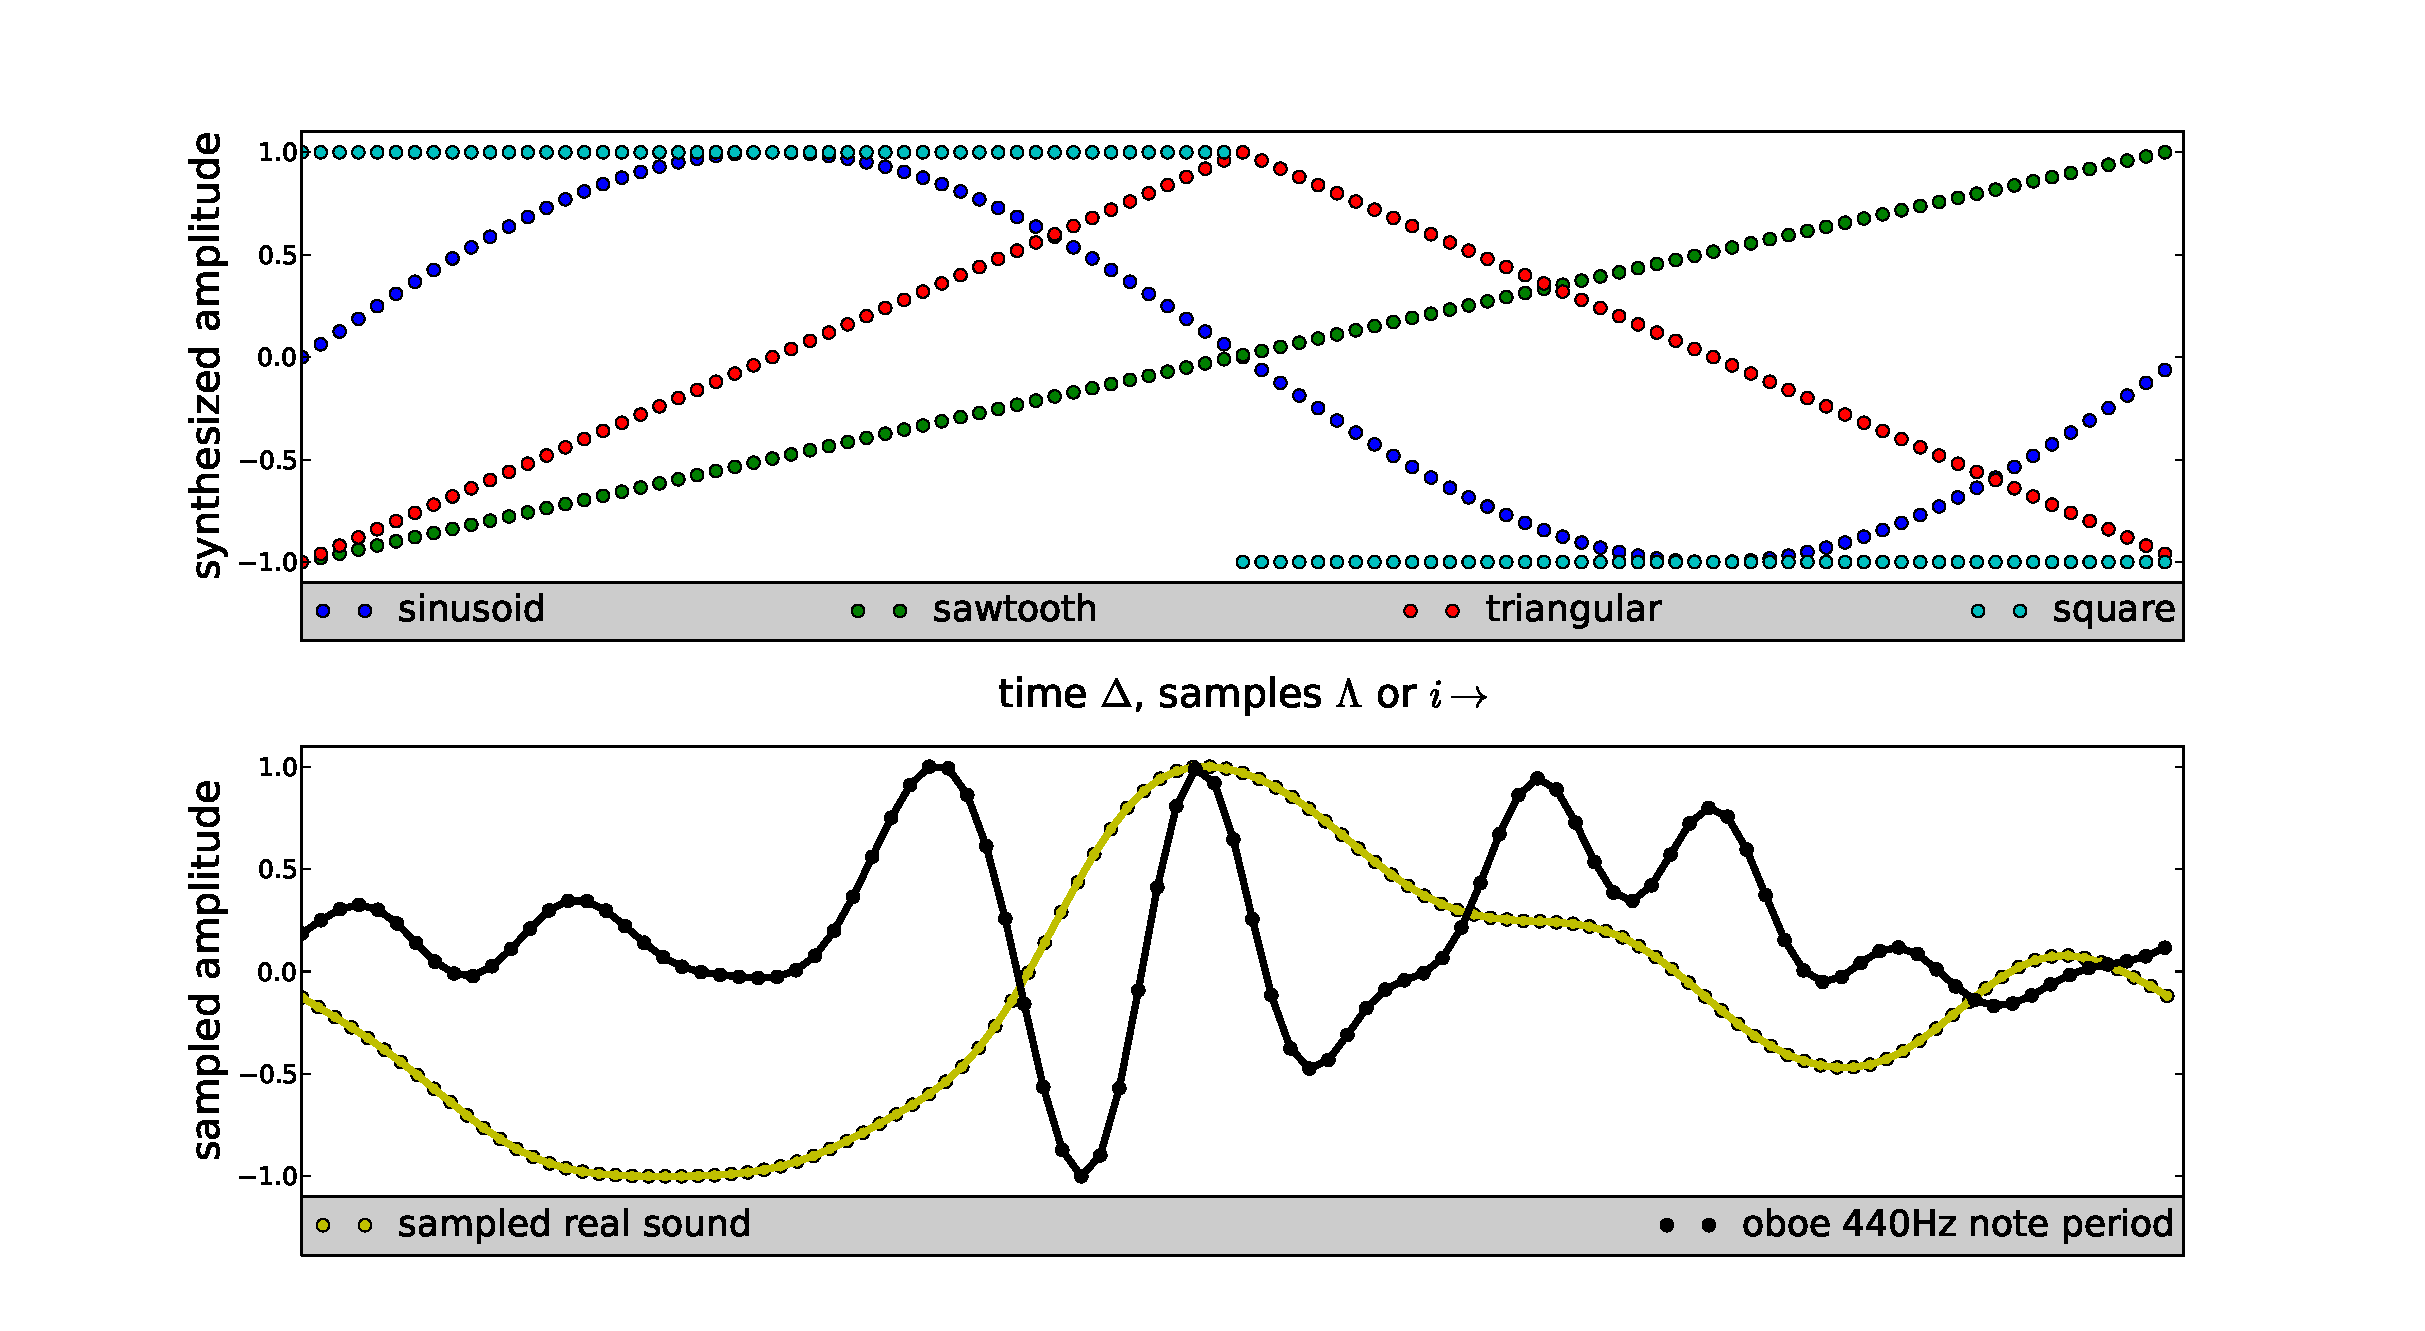
\includegraphics[width=\textwidth]{figures/waveForms}
    \caption{Basic musical waveforms. The synthetic  waveforms are in (a) and the real waveforms are in (b).}
        \label{fig:formasDeOnda}
\end{figure*}

Figure~\ref{fig:formasDeOnda} presents the waveforms described in equations  ~\ref{senoide}, ~\ref{denteDeSerra}, ~\ref{triangular} and ~\ref{quadrada} for $\lambda_f=100$ (period of $100$ samples). If $f_s=44.1kHz$, as PCM standard in Compact Disks, the wave has fundamental frequency $f=\frac{f_a}{\lambda_f}=\frac{44100}{100} = 441 \; Herz$, an A4, just above the central "C", whatever the waveform is.

The spectrum of each basic waveform is in figure~\ref{fig:espectroDeondas}. The isolated and exaclty harmonic components of the spectrum is a consequence of the fixed period usage. The sinusoid consists of a one and only node in spectrum, pure frequency. The sawtooh is the only with a complete harmonic series (odd and even components). Triangular and square waves has the same components (odd harmonics), decaing at $-12dB/octave$ and $-6dB/octave$ respectivelly.

\begin{figure*}
    \centering
        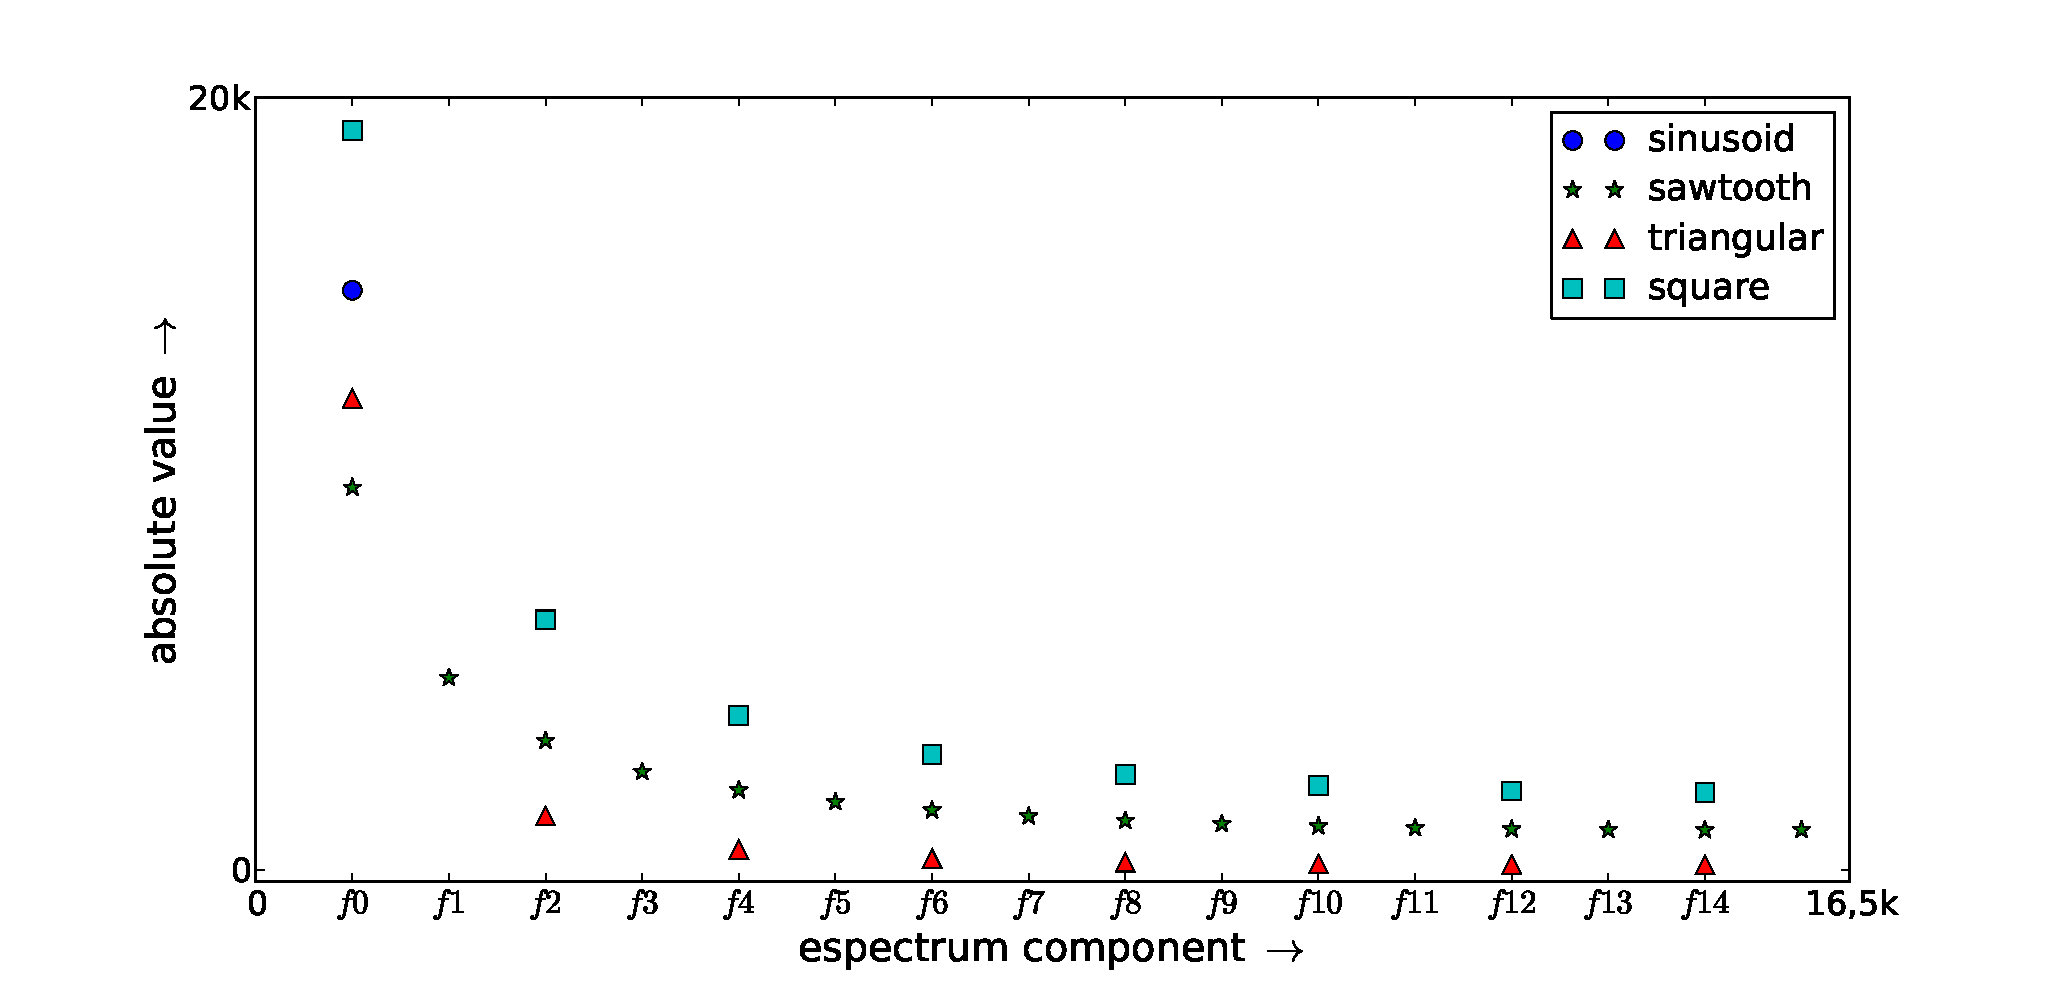
\includegraphics[width=\textwidth]{figures/waveSpectrum}
    \caption{Spectrum of basic artificial musical waveforms.}
        \label{fig:espectroDeOndas}
\end{figure*}

The harmonic spectrum is formed by frequencies multiple from the fundamental frequency $f_n=(n+1)f_0$. As the human linear perception of pitch follows the a geometric progression of frequencies, the spectrum has notes different from the fundamental frequency. Additionally, the number of harmonics will be limited to the maximum frequency $f_s/2$ (by Nyquist's theorem).

Musically crucial here is to internalize that energy in an component of frequency $f_n$ means an oscilation in the constitution of the sound, purely harmonic and in that frequency $f_n$. This energy, specificaly concentrated on the $f_n$ is separated by the ear to enter a cognitive level of processing (this separation is done in many species is mechanisms similar to the human cochlea)~\cite{Roederer}.
The sinusoidal components are usually the main responsibles for the quality we call timbre. If they are not presented in harmonic proportions (small number relations), the sound is perceived as noisy or dissonant and not as a sonority with a univocally stablished fundamental frequency. Furthermore, the notion of absolute pitch in a complex sonority is based relies on the similarity of the spectrum to the harmonic series~\cite{Roederer}.

In the case of a fixed length period and waveform, the spectrum is perfectly harmonic and static. Each waveform is compound of specific proportions of harmonic components and the greater the curvature of a the part, the greater the contribution of the part to the energy on the high harmonics. That can be seen on real sounds. The wave rotulated as ``sampled real sound'' in figure~\ref{fig:formasDeOnda} is a period of $\Lambda_f=114$ samples, extracted from a relatively well behaved real sound. The oboe wave was sampled of a A4 also in $44.1kHz$. The chose period for sampling was a relatively short, with $98$ samples, corresonds to the frequency $\frac{44100}{98}=450Hz$. It can be noticed, from the curvatures, the oboe's rich spectrum in high frequencies and the lower spectrum of the real sound.

The sequence 
$ R_i=\{ r_i \}_0^{\lambda_f-1}$ of samples in the real sound of figure~\ref{fig:formasDeOnda} can be taken as a basis for a sound $T_i^f$ din the following way: 

\begin{equation}\label{sampleandoFormaDeOnda}
     T^f_i=\{ t_i^f \}=\Bigl\{ r_{(i\,\%\lambda_{f})} \Bigr\}
\end{equation}

The resulting sound has a the momentary spectrum of the original sound. Because it is repeated in an identical form, the spectrum is perfectly harmonic, withoud noise and variations tipical of the natural phenomenon.  This can be seen in figure~\ref{fig:espectroOboe}, that show the spectrum of the original oboe note and a note with same duration and whose samples consists of the repetition of cycle of figure~\ref{fig:formasDeOnda}. The natural spectrum exibit variations in the frequencies of the harmonics, its intensities and some noise. The note made from the sampled period has a perfecly harmonic spectrum

\begin{figure*}
    \centering
        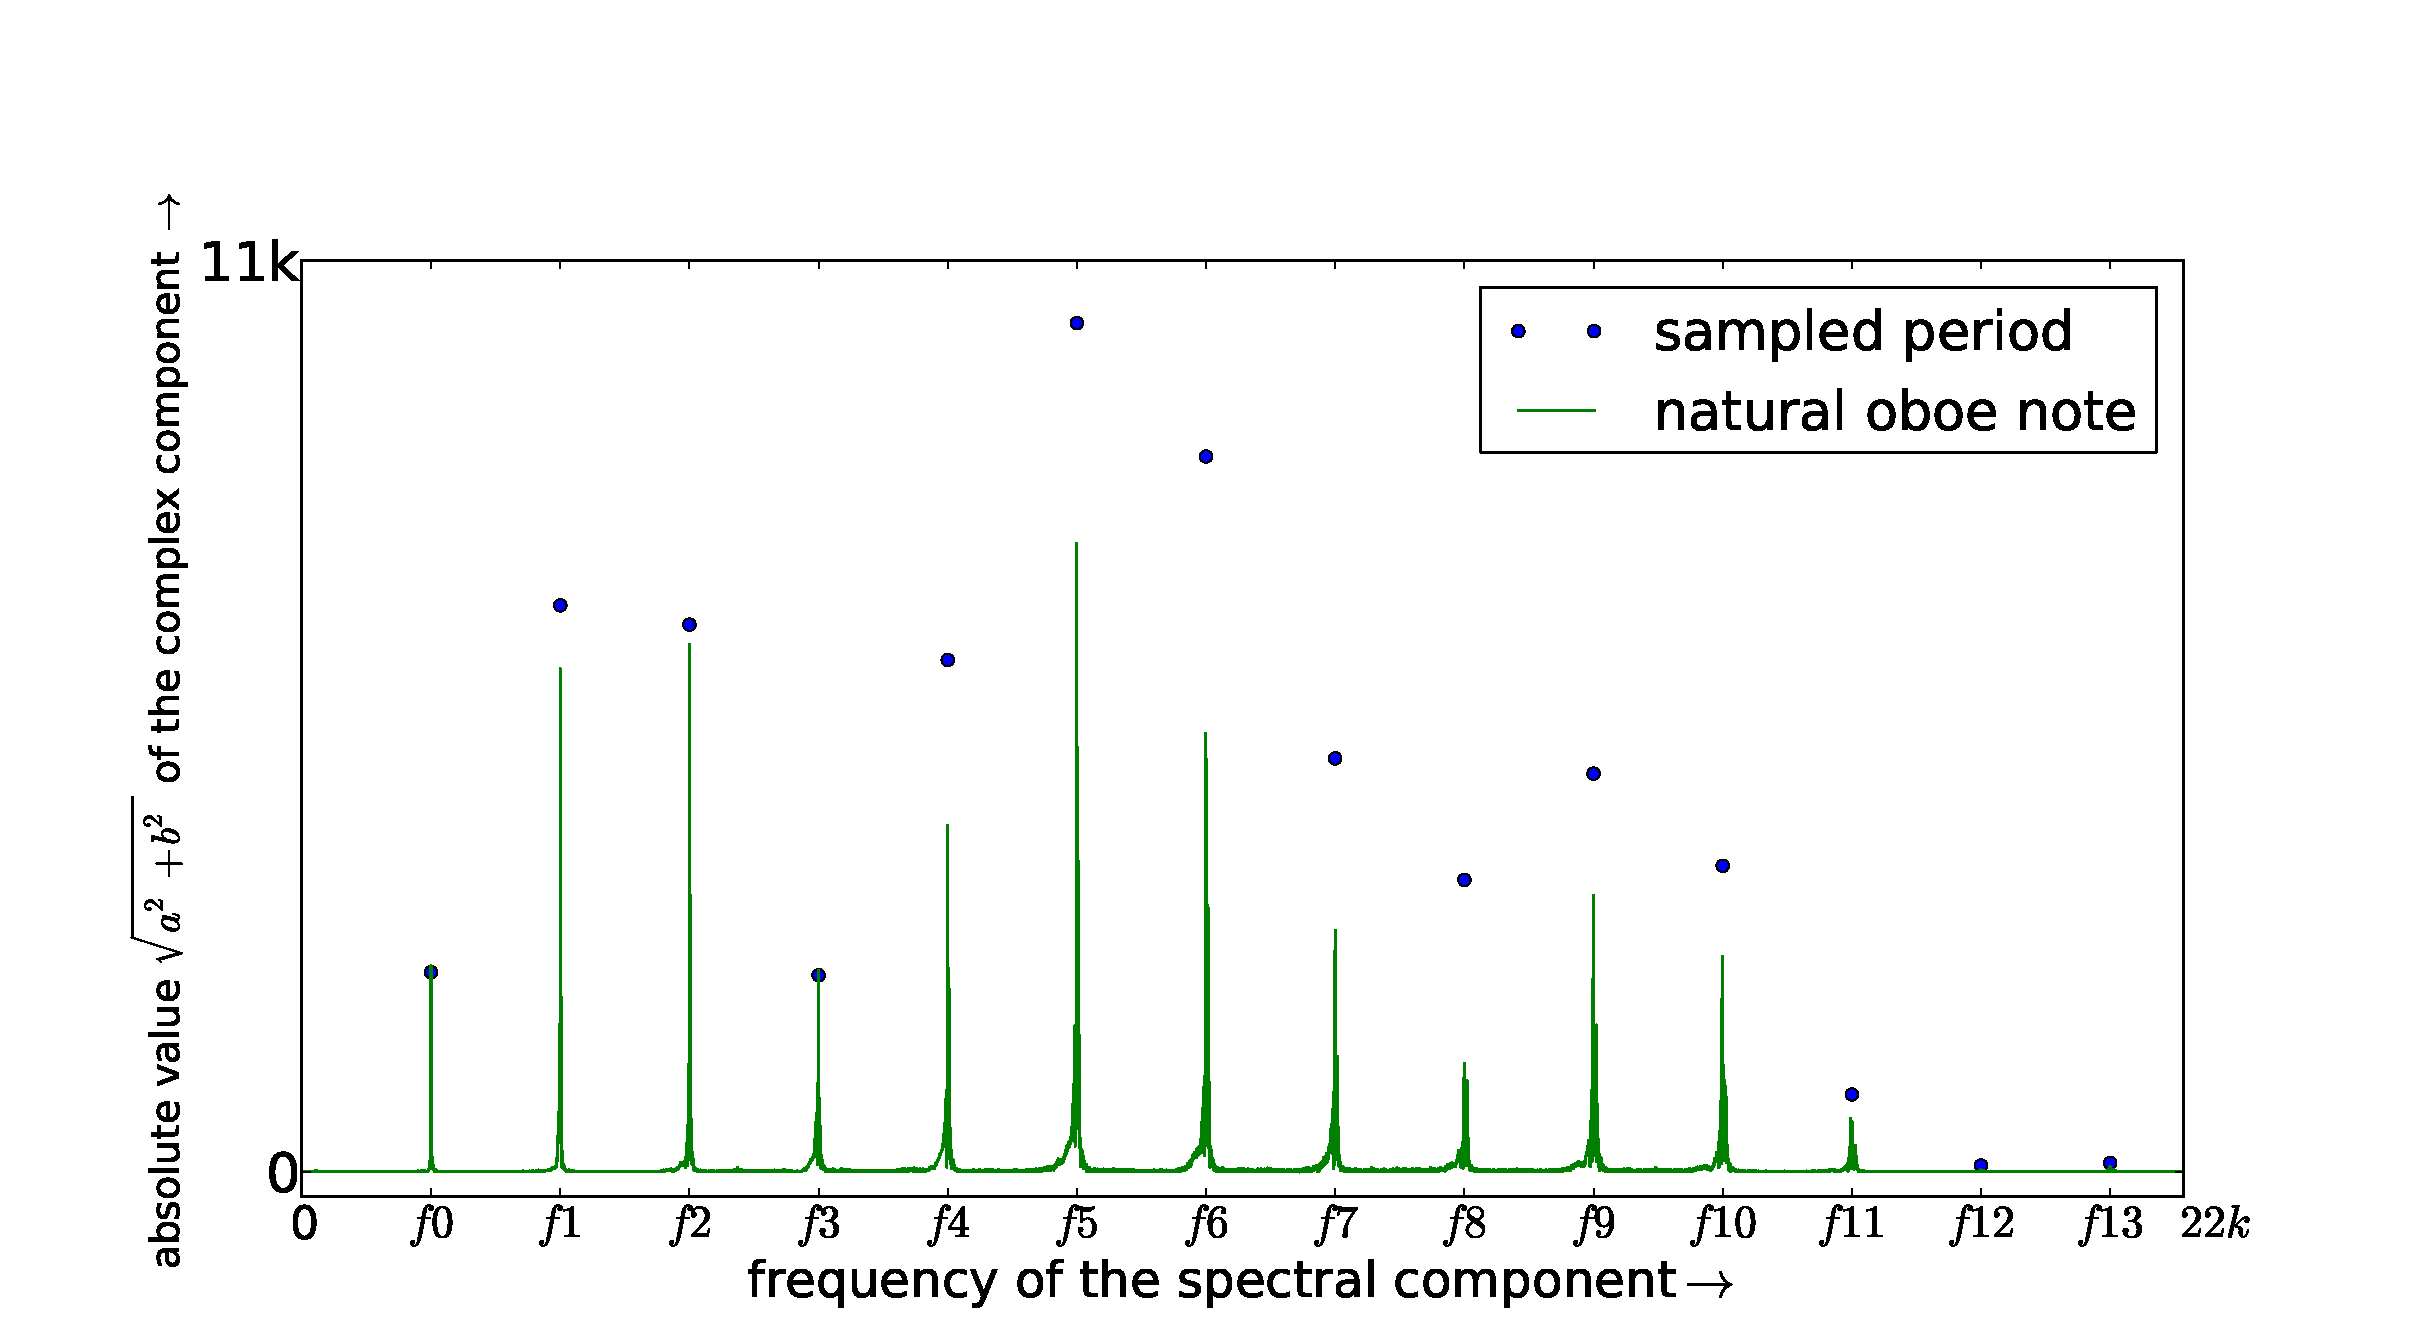
\includegraphics[width=\textwidth]{figures/oboeNaturalSampledSpectrum}
    \caption{Spectrum of the sonic waves of a natural oboe note and one made from a sampled period. The natural sound has fluctuations in the harmonics and in noise, while the sampled period note has a perfectly harmonic spectrum.}
        \label{fig:espectroOboe}
\end{figure*}



\nocite{*}
\bibliography{phi+mus}
\end{document}
